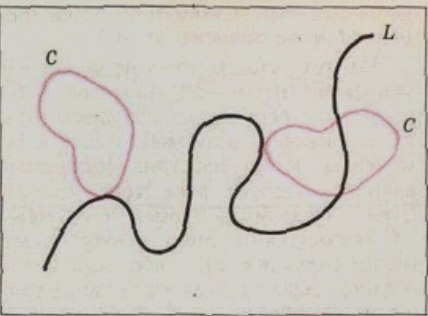
\includegraphics[width=230pt]{main/figure.jpg}

Рис. 8. «Неподвижный рельс» (L) и «колесо» (C).

ное движение можно получить, если рассмотреть качение без скольжения нашего кривого «колеса» по кривому «рельсу» и вовлечь в это качение остальные точки (рис. 8). Будем при этом считать, что отсутствие скольжения означает равенство нулю мгновенных скоростей в точках соприкосновения «колеса» и направляющего «рельса» во все моменты времени (это согласуется с определением мгновенного центра вращения). Отсюда можно вывести равенство длин дуги «колеса» и соответствующей дуги направляющего «рельса» (по которой эта дуга «колеса» прокатилась»). При этом разрешается, чтобы при качении «колесо» пересекало «рельс».

Часто под рулеттами понимают траектории, которые описывают точки плоскости при ее движении как твердой пластины с условием (б) во все моменты времени, то есть при некотором качении. Ко всем рулеттам мы научились проводить нормали и касательные. При этом оказалось, что не нужно даже уметь проводить касательные к «колесу» и «рельсу» (это было бы необходимо, если пользоваться сложением скоростей). В наших механических рассмотрениях мы вышли за пределы XVII века; замечательно, однако, что способ проведения нормалей к общим рулеттам открыл Декарт, определивший их при помощи качения (не зная, конечно, сколь общий характер носят движения, порожденные качениями).

Эпициклоиды

Рассмотрим теперь рулетты, получающиеся при качении круга по кругу. Пусть круг радиуса r катится по внешней стороне окружности радиуса R. Траектории граничных точек катящегося круга («колеса») называются эпициклоидами. Их вид зависит от \(k = R/r\) (рис. 9). Если k — целое, то подвижный круг, прокатившись один раз по границе неподвижного, сделает k оборотов и эпициклоида будет иметь k остриев и k арок. Эпициклоиду приk = 1 называют кардиоидой (она напоминает стилизованное изображение сердца). Если \(k = p/q\) — несократимая дробь, то подвижный круг, сделав q оборотов, p раз прокатится по неподвижному. Если же k будет иррациональным числом, то никакой периодичности не будет, и наблюдаемая точка никогда не вернется в исходное положение.

Можно доказать, что получающаяся в этом случае бесконечная траектория заполняет кольцо

, подходя сколь угодно близко к любой его точке, но не в каждую попадая.

Касательные к эпициклоидам легко строятся с помощью мгновенного центра вращения — точки соприкосновения кругов. Докажите, что касательная к эпициклоиде (в некоторой точке) проходит через точку соответствующего подвижного круга, диаметрально противоположную точке соприкосновения с неподвижным.

Замечание. При построении эпициклоид и решении задач нужно помнить следующее. Если *A* — начальное положение наблюдаемой точки (рис. 10), а в некоторый момент времени подвижный круг касается неподвижного в точке *B*, то эпициклоиде принадлежит такая точка его границы *C*, что дуга *BA* равна по длине дуге *BC*; учитывая разницу радиусов, получаем

\[
\frac{\smile BC}{\smile BA} = \frac{R}{r} = k.
\]

Траектории движения внутренних (соответственно внешних) точек подвижного круга при рассматриваемом качении называются укороченными (соответственно удлиненными) эпициклоидами (рис. 11; мы ограничиваемся целыми k).

\[
\sum_{k,l,m,n,... \ge 0} \frac{1}{2^k 3^l 5^m 7^n ...} = \sum_n \frac{1}{n}
\]
